\documentclass[12pt,letterpaper]{article}
\usepackage[margin=15mm,top=22mm,bottom=18mm,headheight=14pt,headsep=10pt]{geometry}
\usepackage[T1]{fontenc}
\usepackage{helvet}
\renewcommand{\familydefault}{\sfdefault}
\usepackage{tikz}
\usetikzlibrary{arrows.meta}
\usepackage{fancyhdr}
\pagestyle{fancy}
\fancyhf{}
\newcommand{\band}{Grades 2--5}
\fancyhead[L]{\small Week 59 / Constant width / \band}
\fancyfoot[L]{\footnotesize Bellingham Math Circle / Week 59 / W59-S-v4}
\fancyfoot[R]{\footnotesize\thepage}
\renewcommand{\headrulewidth}{0pt}
\renewcommand{\footrulewidth}{0pt}
\setlength{\parindent}{0pt}
\setlength{\parskip}{7pt}
\newcommand{\problem}[2]{\textbf{Problem #1:} #2\par}
\newcommand{\spacebox}[1]{\vspace{3mm}\begin{tikzpicture}[x=1mm,y=1mm]\draw[gray!45,line width=.4pt] (0,0) rectangle (180,#1);\end{tikzpicture}\par}
\begin{document}
\fontsize{12.5}{15.5}\selectfont

To measure width, keep the two straight edges parallel, enclosing the whole piece and just touching it. Turn and slide the piece freely. Measure the perpendicular gap, to the nearest millimeter. This gap is the width in that position. Drawings are smaller than the real pieces.

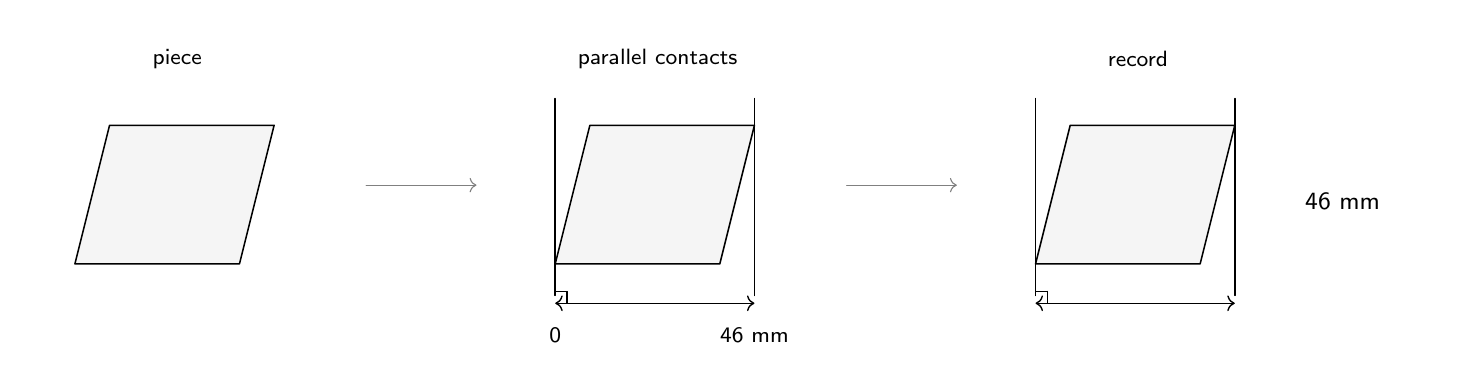
\begin{tikzpicture}[x=1mm,y=1mm,line cap=round,line join=round]
\path[use as bounding box] (0,0) rectangle (180,40);
\draw[fill=gray!8,line width=.55pt] (6.000000000,10.000000000) -- (26.900000000,10.000000000) -- (31.300000000,27.600000000) -- (10.400000000,27.600000000) -- cycle;
\node[font=\footnotesize,inner sep=1pt,] at (19.000000000,36.000000000) {piece};
\draw[fill=gray!8,line width=.55pt] (67.000000000,10.000000000) -- (87.900000000,10.000000000) -- (92.300000000,27.600000000) -- (71.400000000,27.600000000) -- cycle;
\draw[line width=.55pt] (67.000000000,6.000000000) -- (67.000000000,31.000000000);
\draw[line width=.55pt] (92.300000000,6.000000000) -- (92.300000000,31.000000000);
\draw[<->,line width=.5pt] (67.000000000,5.000000000) -- (92.300000000,5.000000000);
\draw[line width=.4pt] (68.500000000,5.000000000) -- (68.500000000,6.500000000);
\draw[line width=.4pt] (67.000000000,6.500000000) -- (68.500000000,6.500000000);
\node[font=\footnotesize,inner sep=1pt,] at (67.000000000,1.000000000) {0};
\node[font=\footnotesize,inner sep=1pt,] at (92.300000000,1.000000000) {46 mm};
\node[font=\footnotesize,inner sep=1pt,] at (80.000000000,36.000000000) {parallel contacts};
\draw[fill=gray!8,line width=.55pt] (128.000000000,10.000000000) -- (148.900000000,10.000000000) -- (153.300000000,27.600000000) -- (132.400000000,27.600000000) -- cycle;
\draw[line width=.55pt] (128.000000000,6.000000000) -- (128.000000000,31.000000000);
\draw[line width=.55pt] (153.300000000,6.000000000) -- (153.300000000,31.000000000);
\draw[<->,line width=.5pt] (128.000000000,5.000000000) -- (153.300000000,5.000000000);
\draw[line width=.4pt] (129.500000000,5.000000000) -- (129.500000000,6.500000000);
\draw[line width=.4pt] (128.000000000,6.500000000) -- (129.500000000,6.500000000);
\node[font=\small,inner sep=1pt,] at (167.000000000,18.000000000) {46 mm};
\node[font=\footnotesize,inner sep=1pt,] at (141.000000000,36.000000000) {record};
\draw[->,gray] (43.000000000,20.000000000) -- (57.000000000,20.000000000);
\draw[->,gray] (104.000000000,20.000000000) -- (118.000000000,20.000000000);
\end{tikzpicture}\par

\problem{1}{Use the five pieces. Find positions that make each gap as small and as large as you can. Keep a sketch and the gap for each.}

\begin{tikzpicture}[x=1mm,y=1mm,line cap=round,line join=round]
\path[use as bounding box] (0,0) rectangle (180,134);
\draw[line width=.45pt] (0.000000000,0.000000000) -- (180.000000000,0.000000000) -- (180.000000000,134.000000000) -- (0.000000000,134.000000000) -- cycle;
\draw[line width=.4pt] (56.000000000,0.000000000) -- (56.000000000,134.000000000);
\draw[line width=.4pt] (118.000000000,0.000000000) -- (118.000000000,134.000000000);
\draw[line width=.4pt] (0.000000000,125.000000000) -- (180.000000000,125.000000000);
\draw[line width=.4pt] (0.000000000,100.000000000) -- (180.000000000,100.000000000);
\draw[line width=.4pt] (0.000000000,75.000000000) -- (180.000000000,75.000000000);
\draw[line width=.4pt] (0.000000000,50.000000000) -- (180.000000000,50.000000000);
\draw[line width=.4pt] (0.000000000,25.000000000) -- (180.000000000,25.000000000);
\node[font=\footnotesize,inner sep=1pt,text width=59mm,align=center] at (87.000000000,129.500000000) {smallest gap};
\node[font=\footnotesize,inner sep=1pt,text width=59mm,align=center] at (149.000000000,129.500000000) {largest gap};
\draw[line width=.55pt,fill=white] (15.000000000,112.500000000) circle (6.600000000);
\node[font=\footnotesize,inner sep=1pt,anchor=west,text width=25mm,align=left] at (28.000000000,112.500000000) {disk};
\draw[line width=.55pt,fill=white] (15.000000000,87.500000000) ellipse (6.600000000 and 4.400000000);
\node[font=\footnotesize,inner sep=1pt,anchor=west,text width=25mm,align=left] at (28.000000000,87.500000000) {oval};
\draw[line width=.55pt,fill=white] (8.400000000,55.900000000) -- (21.600000000,55.900000000) -- (21.600000000,69.100000000) -- (8.400000000,69.100000000) -- cycle;
\node[font=\footnotesize,inner sep=1pt,anchor=west,text width=25mm,align=left] at (28.000000000,62.500000000) {square};
\draw[line width=.55pt,fill=white] (8.400000000,33.689488223) -- (21.600000000,33.689488223) -- (15.000000000,45.121023553) -- cycle;
\node[font=\footnotesize,inner sep=1pt,anchor=west,text width=25mm,align=left] at (28.000000000,37.500000000) {straight\\triangle};
\draw[line width=.55pt,fill=white] (21.600000000,8.689488223) arc[start angle=0.000000000,end angle=60.000000000,radius=13.200000000] arc[start angle=120.000000000,end angle=180.000000000,radius=13.200000000] arc[start angle=240.000000000,end angle=300.000000000,radius=13.200000000] -- cycle;
\node[font=\footnotesize,inner sep=1pt,anchor=west,text width=25mm,align=left] at (28.000000000,12.500000000) {curved\\triangle};
\end{tikzpicture}\par

\newpage

\renewcommand{\band}{Grades K--5}

\problem{2}{Close the edges on the disk, then keep them fixed while the piece turns and slides. Which pieces can turn all the way around inside them? Which can keep touching both edges throughout the turn? Keep a sketch of a deciding position.}

\begin{tikzpicture}[x=1mm,y=1mm,line cap=round,line join=round]
\path[use as bounding box] (0,0) rectangle (180,167);
\draw[line width=.45pt] (0.000000000,0.000000000) -- (180.000000000,0.000000000) -- (180.000000000,167.000000000) -- (0.000000000,167.000000000) -- cycle;
\draw[line width=.4pt] (56.000000000,0.000000000) -- (56.000000000,167.000000000);
\draw[line width=.4pt] (99.000000000,0.000000000) -- (99.000000000,167.000000000);
\draw[line width=.4pt] (142.000000000,0.000000000) -- (142.000000000,167.000000000);
\draw[line width=.4pt] (0.000000000,155.000000000) -- (180.000000000,155.000000000);
\draw[line width=.4pt] (0.000000000,124.000000000) -- (180.000000000,124.000000000);
\draw[line width=.4pt] (0.000000000,93.000000000) -- (180.000000000,93.000000000);
\draw[line width=.4pt] (0.000000000,62.000000000) -- (180.000000000,62.000000000);
\draw[line width=.4pt] (0.000000000,31.000000000) -- (180.000000000,31.000000000);
\node[font=\footnotesize,inner sep=1pt,text width=37mm,align=center] at (77.500000000,161.000000000) {turn inside?};
\node[font=\footnotesize,inner sep=1pt,align=center] at (120.500000000,161.000000000) {touch both\\throughout?};
\node[font=\footnotesize,inner sep=1pt,align=center] at (161.000000000,161.000000000) {deciding\\position};
\draw[line width=.55pt,fill=white] (15.000000000,139.500000000) circle (6.600000000);
\node[font=\footnotesize,inner sep=1pt,anchor=west,text width=25mm,align=left] at (28.000000000,139.500000000) {disk};
\draw[line width=.55pt,fill=white] (15.000000000,108.500000000) ellipse (6.600000000 and 4.400000000);
\node[font=\footnotesize,inner sep=1pt,anchor=west,text width=25mm,align=left] at (28.000000000,108.500000000) {oval};
\draw[line width=.55pt,fill=white] (8.400000000,70.900000000) -- (21.600000000,70.900000000) -- (21.600000000,84.100000000) -- (8.400000000,84.100000000) -- cycle;
\node[font=\footnotesize,inner sep=1pt,anchor=west,text width=25mm,align=left] at (28.000000000,77.500000000) {square};
\draw[line width=.55pt,fill=white] (8.400000000,42.689488223) -- (21.600000000,42.689488223) -- (15.000000000,54.121023553) -- cycle;
\node[font=\footnotesize,inner sep=1pt,anchor=west,text width=25mm,align=left] at (28.000000000,46.500000000) {straight\\triangle};
\draw[line width=.55pt,fill=white] (21.600000000,11.689488223) arc[start angle=0.000000000,end angle=60.000000000,radius=13.200000000] arc[start angle=120.000000000,end angle=180.000000000,radius=13.200000000] arc[start angle=240.000000000,end angle=300.000000000,radius=13.200000000] -- cycle;
\node[font=\footnotesize,inner sep=1pt,anchor=west,text width=25mm,align=left] at (28.000000000,15.500000000) {curved\\triangle};
\end{tikzpicture}\par

\newpage

\renewcommand{\band}{Grades 3--5}
A compass draws an arc with one center and one radius.

\begin{tikzpicture}[x=1mm,y=1mm,line cap=round,line join=round]
\path[use as bounding box] (0,0) rectangle (180,53);
\fill (12.000000000,15.000000000) circle (.55);
\node[font=\footnotesize,inner sep=1pt,] at (9.000000000,13.000000000) {$D$};
\fill (29.500000000,15.000000000) circle (.55);
\node[font=\footnotesize,inner sep=1pt,] at (32.500000000,13.000000000) {$E$};
\fill (12.000000000,32.500000000) circle (.55);
\node[font=\footnotesize,inner sep=1pt,] at (9.000000000,34.500000000) {$F$};
\draw[gray,dashed,line width=.4pt] (12.000000000,15.000000000) -- (29.500000000,15.000000000);
\draw[gray,dashed,line width=.4pt] (12.000000000,15.000000000) -- (12.000000000,32.500000000);
\node[font=\footnotesize,inner sep=1pt,] at (21.000000000,10.000000000) {25 mm};
\node[font=\footnotesize,inner sep=1pt,] at (22.000000000,46.000000000) {given points};
\fill (72.000000000,15.000000000) circle (.55);
\node[font=\footnotesize,inner sep=1pt,] at (69.000000000,13.000000000) {$D$};
\fill (89.500000000,15.000000000) circle (.55);
\node[font=\footnotesize,inner sep=1pt,] at (92.500000000,13.000000000) {$E$};
\fill (72.000000000,32.500000000) circle (.55);
\node[font=\footnotesize,inner sep=1pt,] at (69.000000000,34.500000000) {$F$};
\draw[gray,dashed,line width=.4pt] (72.000000000,15.000000000) -- (89.500000000,15.000000000);
\draw[gray,dashed,line width=.4pt] (72.000000000,15.000000000) -- (72.000000000,32.500000000);
\draw[line width=.8pt] (72.000000000,15.000000000) -- (80.750000000,38.000000000);
\draw[line width=.8pt] (80.750000000,38.000000000) -- (89.500000000,15.000000000);
\draw[line width=.55pt] (80.750000000,38.000000000) circle (1.000000000);
\node[font=\footnotesize,inner sep=1pt,] at (82.000000000,47.000000000) {opening $DE$};
\node[font=\footnotesize,inner sep=1pt,] at (82.000000000,4.000000000) {point at $D$};
\fill (132.000000000,15.000000000) circle (.55);
\node[font=\footnotesize,inner sep=1pt,] at (129.000000000,13.000000000) {$D$};
\fill (149.500000000,15.000000000) circle (.55);
\node[font=\footnotesize,inner sep=1pt,] at (152.500000000,13.000000000) {$E$};
\fill (132.000000000,32.500000000) circle (.55);
\node[font=\footnotesize,inner sep=1pt,] at (129.000000000,34.500000000) {$F$};
\draw[gray,dashed,line width=.4pt] (132.000000000,15.000000000) -- (149.500000000,15.000000000);
\draw[gray,dashed,line width=.4pt] (132.000000000,15.000000000) -- (132.000000000,32.500000000);
\draw[line width=1pt] (149.500000000,15.000000000) arc[start angle=0.000000000,end angle=90.000000000,radius=17.500000000];
\node[font=\footnotesize,inner sep=1pt,] at (142.000000000,46.000000000) {arc $EF$};
\draw[->,gray] (43.000000000,25.000000000) -- (57.000000000,25.000000000);
\draw[->,gray] (103.000000000,25.000000000) -- (117.000000000,25.000000000);
\end{tikzpicture}\par

\problem{3}{Use the 60 mm and 40 mm equilateral templates to make two curved triangles. Each short arc joins two corners and has the third corner as its center. Predict the width of each piece, then test it.}

\begin{tikzpicture}[x=1mm,y=1mm,line cap=round,line join=round]
\path[use as bounding box] (0,0) rectangle (180,90);
\draw[line width=.45pt] (0.000000000,0.000000000) -- (180.000000000,0.000000000) -- (180.000000000,90.000000000) -- (0.000000000,90.000000000) -- cycle;
\draw[line width=.4pt] (90.000000000,0.000000000) -- (90.000000000,90.000000000);
\node[font=\small,inner sep=1pt,] at (45.000000000,82.000000000) {60 mm triangle};
\node[font=\footnotesize,inner sep=1pt,anchor=west] at (7.000000000,66.000000000) {predicted width:};
\node[font=\footnotesize,inner sep=1pt,anchor=west] at (7.000000000,50.000000000) {measured gaps:};
\node[font=\small,inner sep=1pt,] at (135.000000000,82.000000000) {40 mm triangle};
\node[font=\footnotesize,inner sep=1pt,anchor=west] at (97.000000000,66.000000000) {predicted width:};
\node[font=\footnotesize,inner sep=1pt,anchor=west] at (97.000000000,50.000000000) {measured gaps:};
\end{tikzpicture}\par

\spacebox{40}

\newpage

A line that touches a circle at just one point meets the radius there at a right angle.

\begin{tikzpicture}[x=1mm,y=1mm,line cap=round,line join=round]
\path[use as bounding box] (0,0) rectangle (180,46);
\draw[line width=.55pt,fill=white] (26.000000000,24.000000000) circle (12.350000000);
\fill (26.000000000,24.000000000) circle (.55);
\node[font=\footnotesize,inner sep=1pt,] at (23.000000000,21.000000000) {$X$};
\node[font=\footnotesize,inner sep=1pt,] at (26.000000000,5.000000000) {circle};
\draw[line width=.55pt,fill=white] (87.000000000,24.000000000) circle (12.350000000);
\fill (87.000000000,24.000000000) circle (.55);
\node[font=\footnotesize,inner sep=1pt,] at (84.000000000,21.000000000) {$X$};
\draw[line width=.55pt] (67.000000000,36.350000000) -- (107.000000000,36.350000000);
\fill (87.000000000,36.350000000) circle (.55);
\node[font=\footnotesize,inner sep=1pt,] at (90.000000000,39.350000000) {$P$};
\node[font=\footnotesize,inner sep=1pt,] at (87.000000000,5.000000000) {one contact};
\draw[line width=.55pt,fill=white] (148.000000000,24.000000000) circle (12.350000000);
\fill (148.000000000,24.000000000) circle (.55);
\node[font=\footnotesize,inner sep=1pt,] at (145.000000000,21.000000000) {$X$};
\draw[line width=.55pt] (128.000000000,36.350000000) -- (168.000000000,36.350000000);
\fill (148.000000000,36.350000000) circle (.55);
\node[font=\footnotesize,inner sep=1pt,] at (151.000000000,39.350000000) {$P$};
\draw[line width=.55pt] (148.000000000,24.000000000) -- (148.000000000,36.350000000);
\draw[line width=.55pt] (148.000000000,33.850000000) -- (150.500000000,33.850000000);
\draw[line width=.55pt] (150.500000000,33.850000000) -- (150.500000000,36.350000000);
\node[font=\footnotesize,inner sep=1pt,] at (148.000000000,5.000000000) {right angle};
\draw[->,gray] (49.000000000,24.000000000) -- (61.000000000,24.000000000);
\draw[->,gray] (110.000000000,24.000000000) -- (122.000000000,24.000000000);
\end{tikzpicture}\par

\problem{4}{Explain why the exact curved triangle has the same width in every direction. Its arcs have radius 60 mm, with centers at $A$, $B$ and $C$. Your explanation should also work for every position between the drawings.}

\begin{tikzpicture}[x=1mm,y=1mm,line cap=round,line join=round]
\path[use as bounding box] (0,0) rectangle (180,65);
\draw[line width=.55pt,fill=white] (47.537972923,24.555572167) arc[start angle=7.000000000,end angle=67.000000000,radius=33.000000000] arc[start angle=127.000000000,end angle=187.000000000,radius=33.000000000] arc[start angle=247.000000000,end angle=307.000000000,radius=33.000000000] -- cycle;
\draw[gray,densely dashed,line width=.35pt] (14.783949919,20.533883835) -- (47.537972923,24.555572167);
\draw[gray,densely dashed,line width=.35pt] (47.537972923,24.555572167) -- (27.678077159,50.910543998);
\draw[gray,densely dashed,line width=.35pt] (27.678077159,50.910543998) -- (14.783949919,20.533883835);
\fill (14.783949919,20.533883835) circle (.55);
\node[font=\footnotesize,inner sep=1pt,] at (11.749134980,18.246986747) {$A$};
\fill (47.537972923,24.555572167) circle (.55);
\node[font=\footnotesize,inner sep=1pt,] at (51.035891366,23.070793879) {$B$};
\fill (27.678077159,50.910543998) circle (.55);
\node[font=\footnotesize,inner sep=1pt,] at (27.214973654,54.682219375) {$C$};
\draw[line width=.55pt,fill=white] (108.910543998,34.321922841) arc[start angle=37.000000000,end angle=97.000000000,radius=33.000000000] arc[start angle=157.000000000,end angle=217.000000000,radius=33.000000000] arc[start angle=277.000000000,end angle=337.000000000,radius=33.000000000] -- cycle;
\draw[gray,densely dashed,line width=.35pt] (82.555572167,14.462027077) -- (108.910543998,34.321922841);
\draw[gray,densely dashed,line width=.35pt] (108.910543998,34.321922841) -- (78.533883835,47.216050081);
\draw[gray,densely dashed,line width=.35pt] (78.533883835,47.216050081) -- (82.555572167,14.462027077);
\fill (82.555572167,14.462027077) circle (.55);
\node[font=\footnotesize,inner sep=1pt,] at (81.070793879,10.964108634) {$A$};
\fill (108.910543998,34.321922841) circle (.55);
\node[font=\footnotesize,inner sep=1pt,] at (112.682219375,34.785026346) {$B$};
\fill (78.533883835,47.216050081) circle (.55);
\node[font=\footnotesize,inner sep=1pt,] at (76.246986747,50.250865020) {$C$};
\draw[line width=.55pt,fill=white] (161.466116165,47.216050081) arc[start angle=83.000000000,end angle=143.000000000,radius=33.000000000] arc[start angle=203.000000000,end angle=263.000000000,radius=33.000000000] arc[start angle=323.000000000,end angle=383.000000000,radius=33.000000000] -- cycle;
\draw[gray,densely dashed,line width=.35pt] (157.444427833,14.462027077) -- (161.466116165,47.216050081);
\draw[gray,densely dashed,line width=.35pt] (161.466116165,47.216050081) -- (131.089456002,34.321922841);
\draw[gray,densely dashed,line width=.35pt] (131.089456002,34.321922841) -- (157.444427833,14.462027077);
\fill (157.444427833,14.462027077) circle (.55);
\node[font=\footnotesize,inner sep=1pt,] at (158.929206121,10.964108634) {$A$};
\fill (161.466116165,47.216050081) circle (.55);
\node[font=\footnotesize,inner sep=1pt,] at (163.753013253,50.250865020) {$B$};
\fill (131.089456002,34.321922841) circle (.55);
\node[font=\footnotesize,inner sep=1pt,] at (127.317780625,34.785026346) {$C$};
\end{tikzpicture}\par

\spacebox{83}

\newpage

The mark $O$ is a point on a piece. Measure to one straight edge that encloses the whole piece and touches it.

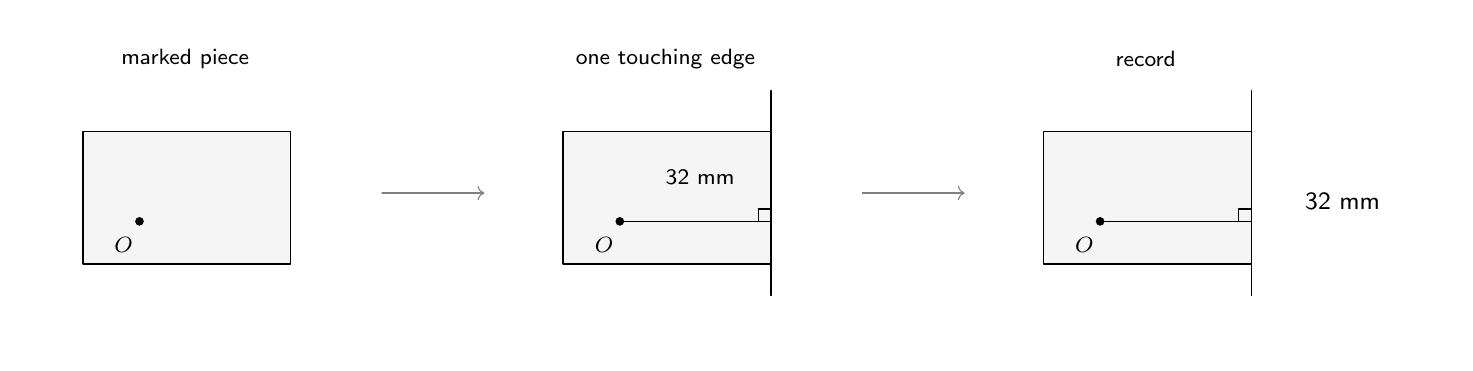
\begin{tikzpicture}[x=1mm,y=1mm,line cap=round,line join=round]
\path[use as bounding box] (0,0) rectangle (180,40);
\draw[fill=gray!8,line width=.55pt] (7.000000000,10.000000000) -- (33.400000000,10.000000000) -- (33.400000000,26.800000000) -- (7.000000000,26.800000000) -- cycle;
\fill (14.200000000,15.400000000) circle (.55);
\node[font=\footnotesize,inner sep=1pt,] at (12.200000000,12.400000000) {$O$};
\node[font=\footnotesize,inner sep=1pt,] at (20.000000000,36.000000000) {marked piece};
\draw[fill=gray!8,line width=.55pt] (68.000000000,10.000000000) -- (94.400000000,10.000000000) -- (94.400000000,26.800000000) -- (68.000000000,26.800000000) -- cycle;
\draw[line width=.55pt] (94.400000000,6.000000000) -- (94.400000000,32.000000000);
\draw[line width=.5pt] (75.200000000,15.400000000) -- (94.400000000,15.400000000);
\draw[line width=.55pt] (92.800000000,15.400000000) -- (92.800000000,17.000000000);
\draw[line width=.55pt] (92.800000000,17.000000000) -- (94.400000000,17.000000000);
\fill (75.200000000,15.400000000) circle (.55);
\node[font=\footnotesize,inner sep=1pt,] at (73.200000000,12.400000000) {$O$};
\node[font=\footnotesize,inner sep=1pt,] at (85.400000000,21.000000000) {32 mm};
\node[font=\footnotesize,inner sep=1pt,] at (81.000000000,36.000000000) {one touching edge};
\draw[fill=gray!8,line width=.55pt] (129.000000000,10.000000000) -- (155.400000000,10.000000000) -- (155.400000000,26.800000000) -- (129.000000000,26.800000000) -- cycle;
\draw[line width=.55pt] (155.400000000,6.000000000) -- (155.400000000,32.000000000);
\draw[line width=.5pt] (136.200000000,15.400000000) -- (155.400000000,15.400000000);
\draw[line width=.55pt] (153.800000000,15.400000000) -- (153.800000000,17.000000000);
\draw[line width=.55pt] (153.800000000,17.000000000) -- (155.400000000,17.000000000);
\fill (136.200000000,15.400000000) circle (.55);
\node[font=\footnotesize,inner sep=1pt,] at (134.200000000,12.400000000) {$O$};
\node[font=\small,inner sep=1pt,] at (167.000000000,18.000000000) {32 mm};
\node[font=\footnotesize,inner sep=1pt,] at (142.000000000,36.000000000) {record};
\draw[->,gray] (45.000000000,19.000000000) -- (58.000000000,19.000000000);
\draw[->,gray] (106.000000000,19.000000000) -- (119.000000000,19.000000000);
\end{tikzpicture}\par

\problem{5}{Use the marked disk and curved triangle. Find the smallest and largest perpendicular distances from $O$ to one touching edge. Can a piece have constant width while those distances change?}

\begin{tikzpicture}[x=1mm,y=1mm,line cap=round,line join=round]
\path[use as bounding box] (0,0) rectangle (180,105);
\draw[line width=.45pt] (0.000000000,0.000000000) -- (180.000000000,0.000000000) -- (180.000000000,105.000000000) -- (0.000000000,105.000000000) -- cycle;
\draw[line width=.4pt] (56.000000000,0.000000000) -- (56.000000000,105.000000000);
\draw[line width=.4pt] (118.000000000,0.000000000) -- (118.000000000,105.000000000);
\draw[line width=.4pt] (0.000000000,96.000000000) -- (180.000000000,96.000000000);
\draw[line width=.4pt] (0.000000000,48.000000000) -- (180.000000000,48.000000000);
\node[font=\footnotesize,inner sep=1pt,text width=59mm,align=center] at (87.000000000,100.500000000) {smallest $O$-to-edge distance};
\node[font=\footnotesize,inner sep=1pt,text width=59mm,align=center] at (149.000000000,100.500000000) {largest $O$-to-edge distance};
\draw[line width=.55pt,fill=white] (15.000000000,72.000000000) circle (6.600000000);
\fill (15.000000000,72.000000000) circle (.55);
\node[font=\footnotesize,inner sep=1pt,] at (18.000000000,69.000000000) {$O$};
\node[font=\footnotesize,inner sep=1pt,anchor=west,text width=25mm,align=left] at (28.000000000,72.000000000) {marked disk};
\draw[line width=.55pt,fill=white] (21.600000000,20.189488223) arc[start angle=0.000000000,end angle=60.000000000,radius=13.200000000] arc[start angle=120.000000000,end angle=180.000000000,radius=13.200000000] arc[start angle=240.000000000,end angle=300.000000000,radius=13.200000000] -- cycle;
\draw[gray,densely dashed,line width=.35pt] (8.400000000,20.189488223) -- (21.600000000,20.189488223);
\draw[gray,densely dashed,line width=.35pt] (21.600000000,20.189488223) -- (15.000000000,31.621023553);
\draw[gray,densely dashed,line width=.35pt] (15.000000000,31.621023553) -- (8.400000000,20.189488223);
\draw[gray,densely dotted,line width=.35pt] (8.400000000,20.189488223) -- (18.300000000,25.905255888);
\draw[gray,densely dotted,line width=.35pt] (21.600000000,20.189488223) -- (11.700000000,25.905255888);
\draw[gray,densely dotted,line width=.35pt] (15.000000000,31.621023553) -- (15.000000000,20.189488223);
\fill (15.000000000,24.000000000) circle (.55);
\node[font=\footnotesize,inner sep=1pt,] at (18.000000000,24.000000000) {$O$};
\node[font=\footnotesize,inner sep=1pt,anchor=west,text width=25mm,align=left] at (28.000000000,24.000000000) {marked curved\\triangle};
\end{tikzpicture}\par

\spacebox{45}

\newpage

\renewcommand{\band}{Grades 4--5}

\problem{6}{Compare the boundary lengths of the 60 mm-width disk and curved triangle. Explain how you know.}

\begin{tikzpicture}[x=1mm,y=1mm,line cap=round,line join=round]
\path[use as bounding box] (0,0) rectangle (180,75);
\draw[line width=.55pt,fill=white] (52.000000000,42.000000000) circle (18.900000000);
\fill (52.000000000,42.000000000) circle (.55);
\draw[line width=.55pt] (52.000000000,42.000000000) -- (70.900000000,42.000000000);
\node[font=\footnotesize,inner sep=1pt,] at (52.000000000,17.000000000) {radius 30 mm};
\node[font=\small,inner sep=1pt,] at (52.000000000,7.000000000) {disk};
\draw[line width=.55pt,fill=white] (146.900000000,31.088079912) arc[start angle=0.000000000,end angle=60.000000000,radius=37.800000000] arc[start angle=120.000000000,end angle=180.000000000,radius=37.800000000] arc[start angle=240.000000000,end angle=300.000000000,radius=37.800000000] -- cycle;
\draw[gray,densely dashed,line width=.35pt] (109.100000000,31.088079912) -- (146.900000000,31.088079912);
\draw[gray,densely dashed,line width=.35pt] (146.900000000,31.088079912) -- (128.000000000,63.823840175);
\draw[gray,densely dashed,line width=.35pt] (128.000000000,63.823840175) -- (109.100000000,31.088079912);
\fill (109.100000000,31.088079912) circle (.55);
\node[font=\footnotesize,inner sep=1pt,] at (105.809103466,29.188079912) {$A$};
\fill (146.900000000,31.088079912) circle (.55);
\node[font=\footnotesize,inner sep=1pt,] at (150.190896534,29.188079912) {$B$};
\fill (128.000000000,63.823840175) circle (.55);
\node[font=\footnotesize,inner sep=1pt,] at (128.000000000,67.623840175) {$C$};
\node[font=\footnotesize,inner sep=1pt,] at (128.000000000,17.000000000) {arcs: radius 60 mm};
\node[font=\small,inner sep=1pt,] at (128.000000000,7.000000000) {curved triangle};
\end{tikzpicture}\par

\spacebox{136}

\end{document}
